\section{Microsoft}
The Xbox line belongs to Microsoft's gaming platforms. It represents a
series of video game consoles developed by Microsoft, with three consoles
released in the sixth, seventh, and eighth generations respectively. The
brand also represents applications (games), streaming services, and an online
service by the name of Xbox Live. The brand was first introduced on November
15, 2001 in the United States, with the launch of the original Xbox
console\cite{Microsoft}.\\

\subsection{Xbox:}
The Xbox is a home video game console and the first installment in the Xbox
series of consoles manufactured by Microsoft. It was released on November 15,
2001, in North America, followed by Australia, Europe and Japan in 2002.
It was Microsoft's first platform into the gaming console market. The
sixth-generation console competed with Sony's PlayStation 2 and the Nintendo
GameCube. It was also the first console produced by an American company since
the Atari Jaguar ceased production in 1996\cite{Microsoft}.\\
The Xbox platform is mostly represented by the \textit{Halo} franchise in
2001 with \textit{Halo: Combat Evolved} with sales of \$6.43 million dollars
and with \textit{Halo 2} in 2004 with \$8.49 million dollars.\\
The total sales for the Xbox platform where \$258.26 million dollars from
2001 to 2008 with 824 games released in total.
\subsection{Xbox 360:}
The Xbox 360 was released as the successor of the original Xbox in November
2005, competing with Sony's PlayStation 3 and Nintendo's Wii as part of the
seventh generation of video game consoles\cite{Microsoft}.\\
Sales-wise, the Xbox 360 performed the best with sales of \$971.63 million
dollars with 1262 registered games under this platform. The most iconic games
for the 360 are \textit{Kinect Adventures!} in 2010 with sales of \$21.81 million
dollars, followed by \textit{Grand Theft Auto V} (2013) with \$16.27 million dollars
in sales and \textit{Call of Duty: Modern Warfare 3} in 2011 with \$14.73
million dollars.
\subsection{Xbox One:}
The Xbox One was released on November 22, 2013 in North America, as the
successor of the Xbox 360. The Xbox One competes with Sony's PlayStation 4
and Nintendo's Wii U as part of the eighth generation of video game
consoles\cite{Microsoft}.\\
This platform is still early to judge with only 3 years in with
sales. According to the dataset there have been sales of \$159.44 million
dollars on 247 released games with the most representative title of
\textit{Call of Duty: Black Ops 3} released in 2015 with 7.39 million
dollars.\\

In order to view with more detail Microsoft's sales please point
\textit{ARMeet} to Figure \ref{fig:MicrosoftImage} and select a platform to view.

\begin{figure}[h]
  \centering
  \centerline{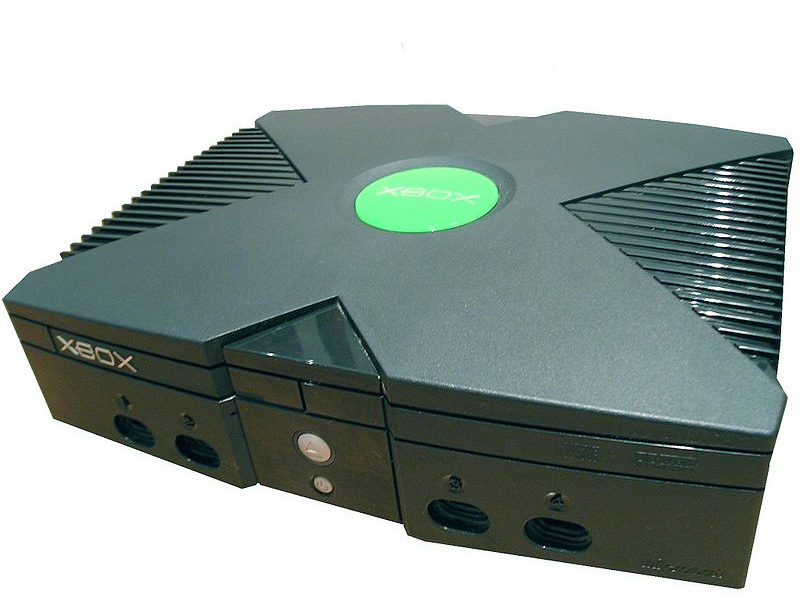
\includegraphics[scale=0.35]{images/MicrosoftMainTarget.png}}
  \caption{Representative picture of Microsoft, point ARMeet to this image to
    see the different sales on each platform.}
  \label{fig:MicrosoftImage}
\end{figure}

%% Platform: XBOX
%% Games: 824
%% Total Sales: 258.2596, by country US: 186.69 EU: 60.94979 JP: 1.38 Other: 8.720057

%% Platform: XBOX360
%% Games: 1262
%% Total Sales: 971.6319, by country US: 602.471 EU: 270.7591 JP: 12.43004 Other: 85.76008

%% Platform: XBOXONE
%% Games: 247
%% Total Sales: 159.44, by country US: 93.12002 EU: 51.59 JP: 0.34 Other: 14.27002
